% $ based on Id: sample_english-v1.2.tex,v 1.2 2007/04/12 21:05:22 zlb Exp $
% $Id: sample_english.tex 6 2011-01-24 13:13:33Z hsqi $

\documentclass[english]{cccconf}
%\documentclass[usemulticol,english]{cccconf}
\usepackage[comma,numbers,square,sort&compress]{natbib}
\usepackage{epstopdf}
\usepackage{comment}
\usepackage{subcaption}
\usepackage{color}
\usepackage{lipsum}
\usepackage{multicol}
\usepackage{amssymb}
\usepackage{amsmath}
\usepackage{bm}
\usepackage{amsfonts}
\usepackage{multirow}
\usepackage{graphicx}
\usepackage{mathtools, amssymb}
\usepackage[comma,numbers,square,sort&compress]{natbib}
\usepackage{CJK}
\usepackage{graphicx}
\usepackage{epsfig}
\usepackage{float}
\usepackage{multirow}
\usepackage{algorithm}
\usepackage{algorithmic}
\usepackage{indentfirst}
\usepackage{booktabs}
\usepackage{amsmath}

\begin{document}

\title{Competition of Social Opinions on Two Layer Networks}

% Note: the first argument in the \affiliation command is optional.
% It defines a label for the affiliation which can be used in the \aref
% command. If there is only one affiliation for all authors, then the
% optional argument in the \affiliation command should be suppressed,
% and the \aref command should also be removed after each author in
% \author command, in this case the affiliation will not be numbered.
% \author{First Author, Second Author, Third Author}
% \affiliation{Chinese Academy of Sciences, Beijing 100190, P.~R.~China\email{ccc@amss.ac.cn}}

\author{Cho Hyunchel \aref{amss,hit},
        A. Mahmood \aref{amss,hit},
        Lin Wang \aref{amss,hit}}
\affiliation[amss]{Department of Automation, Shanghai Jiao Tong University, Shanghai 200240, P.~R.~China}
\affiliation[hit]{Key Laboratory of System Control and Information Processing, Ministry of Education of China, Shanghai 200240, P.~R.~China
        \email{leighsix@naver.com, arfan499@sjtu.edu.cn, wanglin@sjtu.edu.cn}}

\maketitle

\begin{abstract}
Social conflict usually can be investigated based on the competition of two-layers network. In this paper, a competition model is studied on interconnected networks with two-layer opinions, where the first layer is opinion formation and the second layer is decision making. Starting with a polarized competition case where layer A has all the positive opinion and layer B has all the negative opinion, competition simulations are considered with different network structures. With Monte Carlos simulations, different structural models are compared with average state and consensus ratio, which shows that both internal and external links play a vital role for consensus. Especially, increasing the number of external and internal links on one side layer make it easy to reach consensus. However, too many internal edges on each layer make it hard to reach consensus due to inner conflict.
\end{abstract}

\keywords{Interconnected Networks, Opinion Dynamics, Decision Making}

% Please remove or comment out the following line if the footnote is not necessary
\footnotetext{This work was supported by the National Natural Science Foundation of China under Grant Nos 61873167, 61473189, the Natural Science Foundation of Shanghai (No.17ZR1445200).}

\section{Introduction}
In various situations ranging from voting to adoption of new policies, it is widely recognized that opinion formation and decision making formation have mutual interaction as interconnected networks\cite{bianconi2018,domenico2013,tomasini2015, kimsangwoo2012,newman2010,boccaletti2014,mikko2013,huberman2004}. Many researchers have devised many techniques for modeling and analyzing competition on opinion dynamics\cite{amato2017,quattrociocchi2014,haibo2017, hua2014}, voter model\cite{redner2017}, game theory\cite{smyrnakis2019} and many more\cite{danziger2019,namkhanhvu2017,laguna2004,masuda2015,zuev2012, shenyu2018, zhou2018}.  
 
For competition of interconnected networks, many researches have been performed in the various networks, for example the dissemination of computer viruses, messages, opinions, memes, diseases and rumors\cite{hua2014,shenyu2018, zhou2018, alvarez2016,gomez2015,diep2017,rocca2014,velasquez2018}. Opinion dynamics on two-layer or multi-layer networks are investigated, based on \textit{Abrams-Strogatz(AS)} model\cite{abrams2003,vazquez2010} and $M$ model\cite{rocca2014}. Existing research mainly focused on what conditions all agents reach a consensus or dissent, which have shown that the system can make positive consensus, negative consensus or coexistence under certain range of volatility, reinforcement, or prestige. Also, the thresholds or critical points for transition are found to explain and analyze the social phenomena in real world such as the legislation, election result, and social network\cite{alvarez2016, amato2017, diep2017}. In \cite{gomez2015}, it is shown that the transition from localized to mixed status occurs through a cascade from poorly connected nodes in the layers to the highly connected ones. In addition, the main features, such as transition and cascade, found in Monte Carlo simulation are exactly characterized by the mean-field theory and magnetization\cite{alvarez2016, diep2017, amato2017, gomez2015}.   

In this paper, we study the competitions on two interconnected networks with various structures, and investigate which structure has more probability to perform consensus results. With Monte Carlos simulations, consensus of the two-layers network would be compared with different structural models, which shows the vital influence of internal and external links. Specially, when the external links in decision making layer is more than the opinion layer, the tendency to make consensus on both layers is stronger. The more the internal links in one layer is, the stronger the tendency to keep and maintain the state of the layer. However, when each layer has lots of internal links individually, it is hard to make consensus due to inner conflict.    

The paper is organized as follows. In section 2, competition dynamics of interconnected network, that is applied to each layer, is described. In section 3, the simulation results of different structural networks are presented. Lastly, in section 4, the simulation results are summarized.

\section{Modeling}
The model consists of two layers, and each layer has different dynamics. For layer A, the node change its states according to $M$ model as introduced in \cite{rocca2014}. Here, we choose $M=2$, that each node has four states $(-2, -1, +1, +2)$. For each link $(k, j)$ belong to layer A,  the dynamics are designed as follows:
\begin{itemize}
\item Compromise : if two nodes connected with link$(k, j)$ have opposite orientations, their states become more moderate with probability $q$ :
\begin{align*}
\mbox{if } S_k<0 \mbox{ and } S_j>0  \Rightarrow (S_k, S_j) \rightarrow (S_k^r, S_j^l) \mbox{ with } prob.q,\\
\mbox{if } S_k>0 \mbox{ and } S_j<0  \Rightarrow (S_k, S_j) \rightarrow (S_k^l, S_j^r) \mbox{ with } prob.q.
\end{align*}
If $S_k = \pm1$ and $S_j = \mp1$, one switches orientation at random:
\begin{align*}
(\pm 1, \mp 1)\rightarrow \left\{\begin{matrix}
(+1, +1) \mbox{ with } prob.q/2,
\\(-1, -1)\mbox{ with } prob.q/2.
\end{matrix}\right.
\end{align*}
\item Persuasion : if two nodes connected with link$(k, j)$ have the same orientation, their states become more extreme with probability $p$ :
\begin{align*}
\mbox{if } S_k<0 \mbox{ and } S_j<0  \Rightarrow (S_k, S_j) \rightarrow (S_k^l, S_j^l) \mbox{ with } prob.p,\\
\mbox{if } S_k>0 \mbox{ and } S_j>0  \Rightarrow (S_k, S_j) \rightarrow (S_k^r, S_j^r) \mbox{ with } prob.p.
\end{align*}
\end{itemize}
For each external link $(k,j)$ with $k$ belong to layer A, the state of node $k$ is updated according to :
\begin{itemize}
\item $S_k \times S_j < 0$ :
\begin{align*}
\mbox{if } S_k<0 \mbox{ and } S_j>0  \Rightarrow (S_k, S_j) \rightarrow (S_k^r, S_j) \mbox{ with } prob.q,\\
\mbox{if } S_k>0 \mbox{ and } S_j<0  \Rightarrow (S_k, S_j) \rightarrow (S_k^l, S_j) \mbox{ with } prob.q.
\end{align*}
\item $S_k \times S_j > 0$ :
\begin{align*}
\mbox{if } S_k<0 \mbox{ and } S_j<0  \Rightarrow (S_k, S_j) \rightarrow (S_k^l, S_j) \mbox{ with } prob.p,\\
\mbox{if } S_k>0 \mbox{ and } S_j>0  \Rightarrow (S_k, S_j) \rightarrow (S_k^r, S_j) \mbox{ with } prob.p.
\end{align*}
\end{itemize}
Here, $S_k^r$ and $S_k^l$ denote the right and left neighboring states of $k$, defined as
\begin{align*}
S_k^r &= \left\{\begin{matrix}
+1,\mbox{ for } S_k = -1\\
+2,\mbox{ for } S_k = +2\\ 
S_k + 1,\mbox{ otherwise }, 
\end{matrix}\right. &
S_k^l &= \left\{\begin{matrix}
-1,\mbox{ for } S_k= +1
\\ -2,\mbox{ for } S_k=-2
\\ S_k - 1,\mbox{ otherwise }.
\end{matrix}\right.
\end{align*}


The sign of $S^A$ represents its opinion orientation and its absolute value $|S^A|$ measures the intensity of its opinion. So, $|S^A|=2$ represents to a positive or a negative extremist, while  $|S^A|=1$ correspond to a moderate opinion of each side. In case of internal link $(k, j)$ belong to layer A, when the nodes have the same orientation$(S_kS_j>0)$, if the states of nodes are moderate, then they become extreme$(S_k=\pm1 \rightarrow \pm2, S_j= \pm1 \rightarrow \pm2)$ with probability $p$. If they are already extreme, they remain extreme$(S_k=\pm2 \rightarrow \pm2, S_j= \pm2 \rightarrow \pm2)$. On the other hand, when the nodes have opposite orientations$(S_kS_j<0)$, if they are extreme, the states of nodes become moderate$(S_k=\pm2 \rightarrow \pm1, S_j= \pm2 \rightarrow \pm1)$ with probability $q$. If they are already moderate, they switch orientations individually$(S_k=\pm1 \rightarrow \mp1, S_j= \pm1 \rightarrow \mp1)$.  In case of interaction between node in layer A and node in layer B, node in layer A follows opinion dynamics formula, but the state of node in layer B does not change. In other words, the state of layer B affects layer A, but layer A dynamics does not affect the state of node in layer B. For example, one of the layer A node, $S_k = +2$ is connected with  $S_j = -1$ node of layer B. Here, $S_k$ will change into $S_k = +1$ with $prob.q$. But $S_j$ will not change, which indicates that the states of layer B will influence the states of layer A.

The dynamics of layer B follows the decision-making dynamics as introduced in \cite{abrams2003, vazquez2010}. The state of node i in layer B can be $+1$ and $-1$, and it updates according to

\begin{equation}
{P_B}({S_i} \rightarrow - {S_i}) = {\left( {\frac{{{n^{ - {S_i}}}}}{{{i_i} + {e_i}}}} \right)^\beta },
\end{equation}

where $i_i$ is the number of internal edges and $e_i$ is the number of external edges. $n^{-S_i}$ is the number of neighbors of i with opposite state $-S_i$. $\beta(\geq 0)$ is the volatility exponent that measures how prone a node change its state. If $\beta \simeq 0$, a node is very likely to change its state. On the other hand, if $\beta \gg 1$, a node is unlikely to change its state. Also, this formula shows that the more the number of nodes connected with the opposite state is, the easier the nodes are to change into the opposite state.\\
\begin{figure}[!htb]
  \centering
  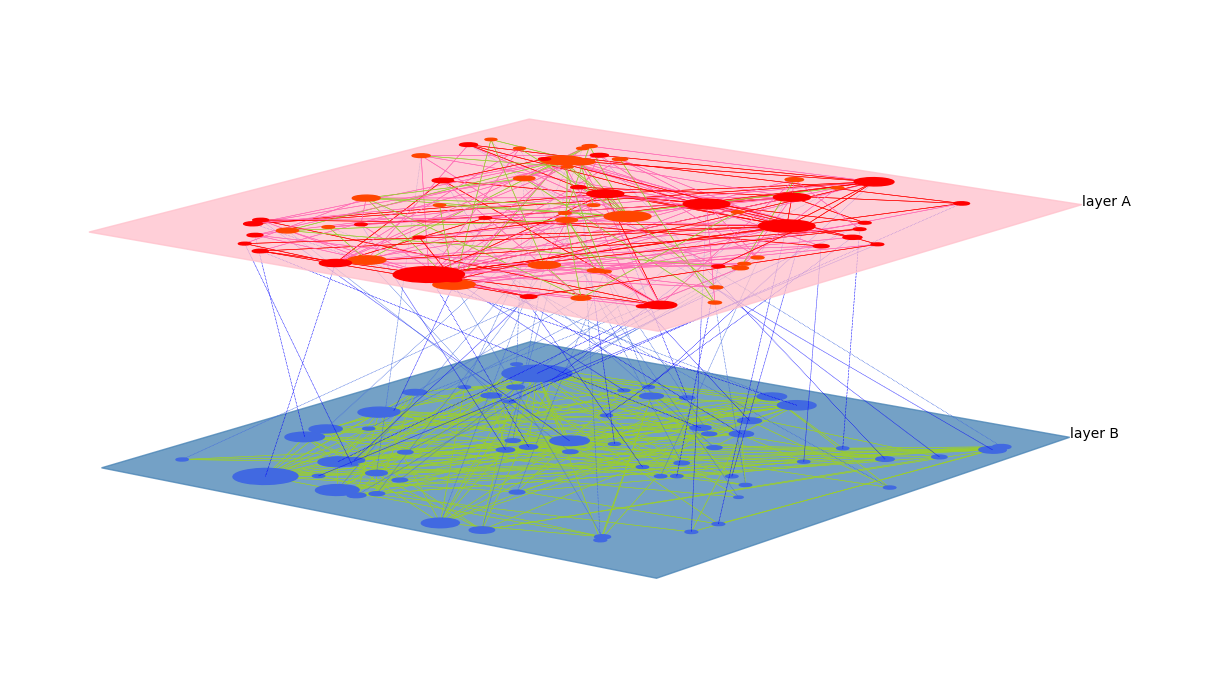
\includegraphics[width=\hsize]{FIG1.png}
  \caption{Competition of Interconnected Network}
  \label{Fig1}
\end{figure}


\section{Simulations and Analysis}
To start with a polarized competition, as the initial conditions,  nodes in layer A are all positive, and nodes in layer B are all negative as shown in Fig(1). For nodes in layer A, it begins with the status where half of nodes are $+1$ and the others are $+2$. The initial state of nodes in layer B have only $-1$. 

There are two parameters in the dynamics of layer A. To simply represent the probability $p$ and probability $q$ together, we set $\gamma = p/q$ based on $p+q=1$. Here, $\gamma$ represents the tendency of opinion such as extreme or moderate, which is scaled to be $0$ to $2$. However, the scale of $\beta$, in the dynamics of layer B, needs to be adjusted, because each model has different links. Based on following Random Regular Networks Model, it would be adjusted to start with the same probability of volatility. 

To implement the interconnected dynamics, one step consists of two layers dynamics, where every node in layer A will be checked with opinion dynamics, and every node in layer B will updates its state according to the decision-making dynamics. Each simulation takes $100$ steps, and $100$ simulations are considered for average results. In the following simulations, we use \textit{`Average State'(AS)} to measure the competition result.

\begin{equation}
AS = avg\left( {\sum\limits_i^{{K^A}} {S_i^A/4} } \right) + avg\left( {\sum\limits_i^{{K^B}} {S_i^B/2} } \right).
\end{equation}

With \textit{AS}, it could be verified whether the consensus happens or not in accordance with the change of $\gamma$ and $\beta$.  If the positive consensus happens, it would be close to the value of $+1$ and if the negative consensus happens, it would be close to the value of $-1$. The values between $+1$ and $-1$ mean the states are belonging to the coexistence part.

\begin{figure*}[!htb]
	\centering
	\includegraphics[width=\hsize]{FIG2.png}
	\caption{(a) $\gamma$-\textit{AS} chart according to certain $\beta$ values. (b) $\beta$-\textit{AS} chart according to certain $\gamma$ values.}
	\label{Fig2}
\end{figure*}

To estimate and evaluate the consensus results regarding different parameters $\gamma$ and $\beta$, we use four kinds of measures including \textit{`AS total'}, \textit{`Positive Consensus Ratio'(PCR)}, \textit{`Negative Consensus ratio'(NCR)}, and \textit{`Consensus Ratio'(CR)}. \textit{AS total} means the summation of \textit{AS} for all $\gamma$s and all $\beta$s. In Eq(3), ${A{S_{{\gamma _i},{\beta _j}}}}$ means $AS$ value with parameters $\gamma_i$ and $\beta_j$, which shows the total orientation and intensity when considering different networks. \textit{PCR} is the ratio of positive consensus over all simulations. Here, positive consensus means  ${A{S_{{\gamma _i},{\beta _j}}} \simeq  1}$. Similarly, \textit{NCR} is the ratio of experiments with negative consensus. \textit{CR} is the ratio of experiments reaching consensus, i.e. summation of \textit{PCR} and \textit{NCR}.

\begin{equation}
\begin{array}{cl}
AS\mbox{ \textit{total} } = \frac{{\sum\limits_j^m {\sum\limits_i^n {A{S_{{\gamma _i},{\beta _j}}}} } }}{{n \times m }}, &
\begin{array}{l}
\gamma  = \left\{ {{\gamma _{\rm{1}}},{\gamma _{\rm{2}}},\left. {\cdot\cdot\cdot,{\gamma _n}} \right\}} \right.\\
\beta {\rm{ = }}\left\{ {{\beta _{\rm{1}}},{\beta _{\rm{2}}},\left. {\cdot\cdot\cdot,{\beta _m}} \right\}} \right.
\end{array}.\
\end{array}
\end{equation}

\begin{equation}
PCR = \frac{{\sum\limits_j^m {\sum\limits_i^n {(A{S_{{\gamma _i},{\beta _j}}} \simeq  1)} } }}{{n \times m}}.
\end{equation}

\begin{equation}
NCR = \frac{{\sum\limits_j^m {\sum\limits_i^n {(A{S_{{\gamma _i},{\beta _j}}} \simeq   - 1)} } }}{{n \times m}}.
\end{equation}

\subsection{Competition on Random Regular Networks}
In this subsection, each layer consists of random regular network that has $N$ nodes with $k$ internal edges as introduced in \cite{kimsangwoo2012, bela2001}. Each node of one layer is connected with a random node on the other layer. This means each node has only $1$ external un-directed edge. Simulations are preformed on network with $N=2048$, and $k = 5$. 

The simulation results are shown in Fig.~\ref{Fig2} and Fig.~\ref{Fig3}. Fig.~\ref{Fig2}(a) shows that when $\gamma > 0.4$, $1.2 < \beta < 1.95$, it normally tends to positive consensus. But, if $\beta$ is lower or larger than certain values, it doesn't make consensus.
In Fig.~\ref{Fig2}(b), as $\beta$ increases, it normally change from positive to negative consensus. But, when $\gamma$ is very low($\gamma \le 0.1$), it doesn't make positive consensus. On the other hand, when $\gamma$ is large enough, it makes positive consensus. But, when $\beta$ is large enough, it is changed into negative consensus. When both of $\gamma$ and $\beta$ are large enough, the state is in a coexistence part.
 
\begin{figure}[!htb]
	\centering
	\includegraphics[width=\hsize]{FIG3.png}
	\caption{Random Regular Networks : \textit{AS} changing with $\gamma$ and $\beta$}
	\label{Fig3}
\end{figure}

Fig.~\ref{Fig3} shows the states of two layers according to all $\gamma$s and all $\beta$s. The $X$-axis is the $\gamma$ and the $Y$-axis is the $\beta$, and the $Z$-axis represents \textit{AS}. The closer the color is to blue, the more it has positive consensus. And the closer the color is to red, the more it has negative consensus. A light and white areas have coexistence with positive states and negative states. This chart has two areas for coexistence, when $\beta$ is very low or very high. When $\beta$ is in certain range, interconnected network can perform positive or negative consensus with different $\gamma$ values.     

\subsection{Competition on Networks with different number of external links}

In this subsection, we consider the influence of external links. Based on the basic model in Subsection 3.1, we reduce the number of nodes in layer B at a certain rate and increase the external links from nodes in layer B accordingly.  We denote \textit{HM(n)} as a hierarchical model with a level $n$, which means that the number of nodes in layer B is $1/n$ of the number of nodes in layer A, and the number of external links from node in layer B is $n$ in view that the number of external links from node in layer A is $1$. In other words, each node in layer A has one external edge, but each node in layer B has $n$ external edges for \textit{HM(n)}, which means one node in layer B can be influenced by $n$ nodes in layer A. $\gamma$ scale is same as the Random Regular Networks Model. But, $\beta$ scale depends on the number of degrees. So the $\beta$ scale is adjusted to have the same probability of volatility with Random Regular Networks Model(\textit{RRM}) as following Equation.
\begin{equation}
{\beta _{h,\max}} = {\beta _{rr,\max}} \cdot \log \left( {\frac{{{n_{rr}}^{ - {S_i}}}}{{{i_{rr,i}} + {e_{rr,i}}}} \cdot \frac{{{i_{h,i}} + {e_{h,i}}}}{{{n_{h}}^{ - {S_i}}}}} \right). 
\end{equation}

Eq(6) is derived from Eq(1) at the initial states. $\beta _{h,\max}$ is the maximum value of $\beta$ scale in \textit{HM}, and $\beta _{rr,\max}$ is the maximum value of $\beta$ scale in \textit{RRM}. When \textit{RRM} begins with initial state and the maximum of $\beta$ scale, it has the lowest volatility except $0$. In order to have the same probability in layer B dynamics for different network structures at the initial time, maximum value of $\beta$ in \textit{HM} is calculated based on Eq(6). 

Fig.~\ref{Fig4} shows the Hierarchical Model simulation results. Comparing \textit{HMs} with \textit{RRM}, \textit{CR} and \textit{PCR} are all increased remarkably. \textit{HMs} have more positive consensus part than \textit{RRM}. It shows that as the number of B nodes are decreased, it is easy to make positive consensus. Comparing \textit{HM(16)} with other \textit{HMs}, \textit{HM(16)} has the most positive consensus part. In case of models where the number of nodes in layer B is less than \textit{HM(16)},  \textit{CR} and \textit{PCR} of the models are decreased and \textit{NCR} is increased slightly. Also, for models where the number of nodes in layer B is more than \textit{HM(16)}, \textit{CR} and \textit{PCR} are also decreased. However, \textit{HM(4)} has the most \textit{AS total}. Although \textit{HM(4)} doesn't have the most consensus part, it has more intensity for positive social opinion. It can be analyzed that strong social intensity usually can not make more consensus. These results indicate that network structure can contribute more for consensus. 
   
\begin{figure}[!htb]
	\centering
	\includegraphics[width=\hsize]{FIG4.png}
	\caption{Hierarchical Model(\textit{HM(n)})}
	\label{Fig4}
\end{figure}

In summary, all the Hierarchical Models have more consensus ratio than Random Regular Networks Model. Among \textit{HMs}, \textit{HM(16)} has the most positive consensus part. When the number of nodes in layer B is more or less than \textit{HM(16)}, \textit{CR} and \textit{PCR} are decreased. This shows that there exists an efficient number for the decision making layer to perform positive consensus.  

\subsection{Competition on Networks with different number of internal links}
\begin{figure}[!htb]
	\centering
	\includegraphics[width=\hsize]{FIG5.png}
	\caption{Comparison of Networks with different internal degrees(\textit{RR(n)-RR(m)}: layer A has random regular network with $n$ internal edges, layer B has random regular network with $m$ internal edges)}
	\label{Fig5}
\end{figure}
Next, the interconnected networks are simulated with different internal degrees in order to define and evaluate the influence of internal degrees. The number of internal degrees on each node is switched to $2$ or $5$.

Fig.~\ref{Fig5} shows the simulation results with changing the number of internal edges. \textit{RR(5)-RR(2)} has the most \textit{PCR}. \textit{RR(2)-RR(5)} has the most \textit{NCR}. When the number of internal edges in layer A are more than layer B, it has more positive consensus. On the other hand, when the number of internal edges in layer B are more than layer A, it has relatively more negative consensus. These results provide that the number of edges on layer A has the tendency to keep positive state, and the number of edges on layer B has the tendency to keep negative state. The number of internal edges have the influence on consensus result and a layer with more internal edges has the tendency to maintain its own state. In case of networks with same internal edges, \textit{RR(2)-RR(2)} has more \textit{PCR} and \textit{AS total} than \textit{RR(5)-RR(5)}. It can be analyzed that \textit{RR(5)-RR(5)} is hard to make consensus, because it has more internal edges to cause inner conflict. Also, \textit{RR(2)-RR(2)} has less \textit{NCR} than \textit{RR(5)-RR(5)}. It shows that the number of internal edges in layer B is more sensitive than layer A. As Eq(1) shows, layer B dynamics can have more various and extreme probabilities when it has more degrees. For example, in case of \textit{RR(2)-RR(2)} with $\beta = 1$, the dynamics starts with $P_B=1/3$ and in case of \textit{RR(5)-RR(5)} with $\beta = 1$, the dynamics starts with $P_B=1/6$.    

\subsection{Competition on Networks with different structures}
So far, each layer of the interconnected network consisted of random regular networks that has the same number of edges for each node. Now, the simulation would be implemented on different network structures. 

\begin{figure}[!htb]
	\centering
	\includegraphics[width=\hsize]{FIG6.png}
	\caption{Comparison of Networks with different structures}
	\label{Fig6}
\end{figure}

Here, we use \textit{Barabasi-Albert network(BA)} structure as introduced in \cite{barabasi1999}. To evaluate the influence of network structure, 5 simulations are implemented with changing network structures. The \textit{BA} network is applied for both layers or switched on each layer. And, because layer A with \textit{BA} network structure has total $10,215$ internal edges, \textit{RR(10)-RR(5)}, under the similar conditions such as the number of nodes and edges, is also simulated. The simulation results are shown in Fig.~\ref{Fig6}. The result of \textit{BA-RR} and \textit{RR(10)-RR(5)} have almost the same features. The gap of \textit{CR} is almost same(less than 0.01). The structure of network make no obvious difference of consensus results. In case of \textit{BA-BA}, the \textit{CR} has the least ratio for consensus. \textit{BA-BA} structure has lots of internal edges on each layer. Therefore, it is hard to make consensus due to inner conflict on each layer. 

\section{Conclusion}
In this work, we have considered competition on interconnected networks, where layer A is a layer of social opinion and layer B is a network representing decision making. When these two layers are connected and interacted, three final states, negative consensus, positive consensus, and coexistence appear according to $\gamma$ and $\beta$. Competition results are measured with \textit{AS total}, \textit{PCR}, \textit{NCR}, and \textit{CR}, which show that interconnected networks with hierarchy help to make consensus, and a layer with more internal edges has more tendency to keep its own states. However, too many internal edges on each layer can cause inner conflict, which makes it hard to reach consensus. As future work, it would be very interesting to make the generalized model for competing interconnected network and find the key nodes and edges of interconnected network.

\begin{thebibliography}{0}
\bibitem{bianconi2018}
G. Bianconi, \textit{Multilayer Networks: Structure and Function}, Oxford University Press, 2018.

\bibitem{domenico2013}
M. De Domenico et al, \textit{Mathematical Formulation of Multilayer Networks}, Physical Review X 3, 041022, 2013.

\bibitem{tomasini2015}
Marcello Tomasini, \textit{An Introduction to Multilayer Networks}, 10.13140/RG.2.2.16830.18243, 2015.

\bibitem{kimsangwoo2012}
Kim Sangwoo, \textit{Structure and dynamics of complex networks}, Yonsei Univ, 2012.

\bibitem{newman2010}
M. E. J. Newman, \textit{Networks: An Introduction}, Oxford University Press, 2010.
	
\bibitem{boccaletti2014}
S. Boccaletti et al, \textit{The structure and dynamics of multilayer networks}, Physics Reports 544, 2014.	

\bibitem{mikko2013}
Mikko Kivela et al, \textit{Multilayer Networks}, J. Complex Networks Volume 2. DOI : 10.1093/comnet/cnu016, 2013.	

\bibitem{huberman2004}
Wu F. and Huberman B.A, \textit{Social structure and opinion formation}, arXiv.org:cond-mat/0407252v3, 2004.	

\bibitem{hua2014}
Hua Jun, Lin Wang, Xiaofan Wang, \textit{An information diffusion model based on individual characteristics}, 33rd Chinese Control Conference (CCC), 2014.

\bibitem{amato2017}
R Amato et al, \textit{Opinion competition dynamics on multiplex networks}, New Journal of Physics volume 19, 2017.

\bibitem{quattrociocchi2014}
Walter Quattrociocchi et al, \textit{Opinion dynamics on interacting networks : media competition and social influence}, Scientific Reports:Complex networks Statistical Physics, 2014.

\bibitem{haibo2017}
Haibo Hu, \textit{Competing opinion diffusion on social networks}, Royal Society Open Science volume 4, 2017.

\bibitem{redner2017}
Sidney Redner, \textit{Dynamics of Voter Models on Simple and Complex Networks}, Physics and Society(physics.soc-ph), 2017.

\bibitem{smyrnakis2019}
Michalis Smyrnakis et al, \textit{An evolutionary game perspective on quantised consensus in opinion dynamics}, PLoS ONE 14(1):e0209212, 2019.

\bibitem{shenyu2018}
Shenyu Zhou, Shuyang Shi, Lin Wang, \textit{Immunizations of Interacting Diseases}, 37rd Chinese Control Conference (CCC), 2018.

\bibitem{zhou2018}
Shenyu Zhou, Shuangdie Xu, Lin Wang, Zhixin Liu, Guanrong Chen, Xiaofan Wang, \textit{Propagation of interacting diseases on multilayer networks}, Physical Review E 98, 2018. 

\bibitem{danziger2019}
Danziger, Michael M. et al, \textit{Dynamic interdependence and competition in multilayer networks}, Nature Physics Volume 15. pp.178-185, 2019.

\bibitem{namkhanhvu2017}
Nam Khanh Vu, \textit{Robustness of Interconnected Complex Networks with Directed Dependency}, Yonsei University Department of Computer Science, 2017.

\bibitem{laguna2004}
M. F. Laguna et al, \textit{The dynamics of opinion in hierarchical organizations}, arXiv.org:nlin/0404024, 2004. 

\bibitem{masuda2015}
Naoki Masuda, \textit{Opinion control in complex networks}, New Journal of Physics, Volume 17, 2015.

\bibitem{zuev2012}
Zuev A S and Fedyanin, 
\textit{Models of opinion control for agents in social networks}, Automation and Remote Control Volume 73 Issue 10, pp.1753–1764, 2012. 

\bibitem{alvarez2016}
Alvarez Zuzek et al, \textit{Interacting Social Processes on Interconnected Network}, PLoS ONE. 11. 10.1371/journal.pone.0163593, 2016.

\bibitem{gomez2015}
Gomez Gardenes J. et al, \textit{Layer-layer competition in multiplex complex network}, Phil. Trans. R. Soc. A 373:20150117, 2015.

\bibitem{diep2017}
H.T. Diep et al, \textit{Dynamics of two-group conflicts: A statistical physics model}, Physica A: Statistical Mechanics and its Applications Volume 467. pp.183 - 199, 2017.

\bibitem{rocca2014}
C. E. La Rocca et al, \textit{The influence of persuasion in opinion formation and polarization}, Europhys. Lett. 106, 40004, pp.1-2, 2014.

\bibitem{velasquez2018}
F. Vel{\'a}zquez et al,\textit{Opinion dynamics in two dimensions: domain coarsening leads to stable bi-polarization and anomalous scaling exponents}, Physics and Society(physics.soc-ph), 2018. 

\bibitem{abrams2003}
M Abrams et al, \textit{Modelling the dynamics of language death}, Nature.424.900. DOI : 10.1038/424900a, 2003.

\bibitem{vazquez2010}
 F. V{\'a}zquez et al, \textit{Agent based models of language competition: macroscopic descriptions and order–disorder transitions}, Journal of Statistical Mechanics: Theory and Experiment P04007, 2010.

\bibitem{bela2001}
 Bela Bollobas, \textit{Random Graphs}, 2nd edition, Cambridge University Press, section 2.4: Random Regular Graphs, 2001.

\bibitem{barabasi1999}
Barabasi A. L., Albert R, \textit{Emergence of Scaling in Random Networks}, Science 286, 509, DOI: 10.1126/science.286.5439.509, 1999.

\end{thebibliography}

\end{document}



































